\documentclass[11pt, english, fleqn, DIV=15, headinclude, BCOR=2cm]{scrreprt}

\usepackage[
    color,
    bibatend,
]{../../header}

\graphicspath{{./}{../Figures/}}

\usepackage{needspace}

\usepackage{mathtools}
\usepackage{listings}

\lstset{
    basicstyle=\small\ttfamily,
}

\hypersetup{
    pdftitle=
}

\newcommand\mot{\textsc{mot}}

\usepackage{longtable}
\usepackage{subcaption}

\usepackage[all]{nowidow}

\subject{Lab report}
\title{Optical frequency doubling}
\subtitle{Experiment A245 -- Universität Bonn}
\author{%
    Martin Ueding \\
    \small{\href{mailto:mu@martin-ueding.de}{mu@martin-ueding.de}}
    \and
    Lino Lemmer \\
    \small{\href{mailto:l2@uni-bonn.de}{l2@uni-bonn.de}}
}

\date{\daterange{2016-05-23}{2016-05-24}}

\publishers{Tutor: Gautam Ramola}

\begin{document}

\maketitle

\begin{abstract}
\end{abstract}

\tableofcontents

\chapter*{Permission to upload}

I, Martin Ueding, would like to scan and upload this lab report with your
corrections to my website \href{http://martin-ueding.de}{martin-ueding.de}.
There, the original lab report as well as the reviewed one will be licensed
under the “\href{http://creativecommons.org/licenses/by-sa/4.0/}{Creative
Commons Attribution-ShareAlike 4.0 International License}”. Is that okay with
you?

Yes $\Box$ \hspace{2cm} No $\Box$

\chapter{Theory}


\section{Generation of hamonics}

\section{Birefringence}

\subsection{Retarder plates}

\section{Phase matching}

\section{Gaussian beams}

\section{Wavelength measurement}

\subsection{Gratings}

\subsection{Michelson interferometer}

\section{Coherence}

\subsection{Coherence length}

\section{Diode laser}
\label{sec:diode_laser}

% TODO Describe elliptical beam shape.

\chapter{Conduction and analysis}

\section{Diode laser classification}

First we want to classify the Laser diode at hand. We have a diode laser which
is mounted behind a safety shutter. One of the characteristics of a diode laser
is the elliptical beam shape as described in Section~\ref{sec:diode_laser}
already. Therefore our setup includes a pair of prisms in order to get a
circular beam cross section. The whole setup including the power meter is shown
in Figure~\ref{fig:fig-1}.

\begin{figure}
    \centering
    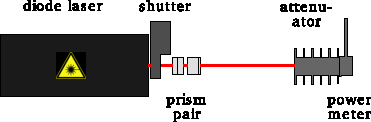
\includegraphics{fig-1}
    \caption{%
        Setup for characterizing the diode laser. Taken from the manual.
    }
    \label{fig:fig-1}
\end{figure}

For measuring the power we just dump the whole beam into a power meter. Since
the power meter become non-linear beyond \SI{20}{\milli\watt} we use an
attenuator in front of it. This will take away a certain fraction of the beam
and allow us to measure higher intensities. The attenuator has to be calibrated
first with small beam powers to allow for a comparison.


% TODO Measure up to 280 mA.
% TODO Measure background.
% TODO Calibrate attenuator.

\subsection{Injection current}

% TODO Plot output versus current.

\subsection{Threshold current}

% TODO Extract threshold.

\subsection{Quantum efficiency}

% TODO Compute differential slope efficiency.
% TODO Compute quantum efficiency from slope.

\subsection{Variable attenuator}

The laser might experience \emph{mode hops} when we adjust the current.
Therefore we do not want to adjust laser power by the current during our
adjustment. We rather want to have an optical way to adjust the beam power. For
this we will use a polarizing beam splitter and a $\lambda/2$-plate in front of
that. By adjusting the polarization of the beam going into the polarizing
splitter we can select the portion of the power advancing to the next parts in
our setup. We extend out setup with a plate and splitter like shown in
Figure~\ref{fig:fig-2}.

\begin{figure}
    \centering
    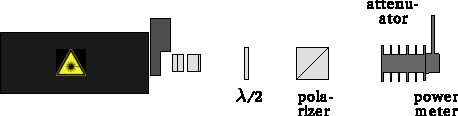
\includegraphics{fig-2}
    \caption{%
        %
    }
    \label{fig:fig-2}
\end{figure}

We must obtain a relation of retarder plate angle and output power to use this
later on. There is only one power meter and we want to measure the powers of
both the fundamental and harmonic beam at the same time. We take power
measurements of the fundamental beam in \SI{2.5}{\degree} steps of the retarder
plate.

% TODO Measure power depending on the retarder plate angle.

We expect to see a $\cos^2$ profile, perhaps with a constant offset.

\section{Harmonic power}

\begin{figure}
    \centering
    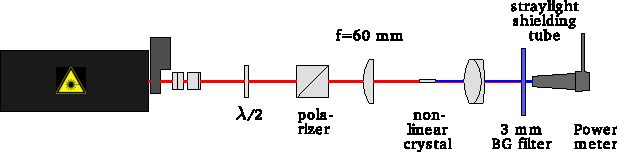
\includegraphics{fig-4}
    \caption{%
        %
    }
    \label{fig:fig-4}
\end{figure}

\subsection{Output power optimization}

\subsection{Crystal temperature dependence}

\subsection{Input power dependence}

\subsection{Input polarization dependence}

\section{Wavelength comparison}

\subsection{Grating}

\subsection{Michelson interferometer}

\begin{figure}
    \centering
    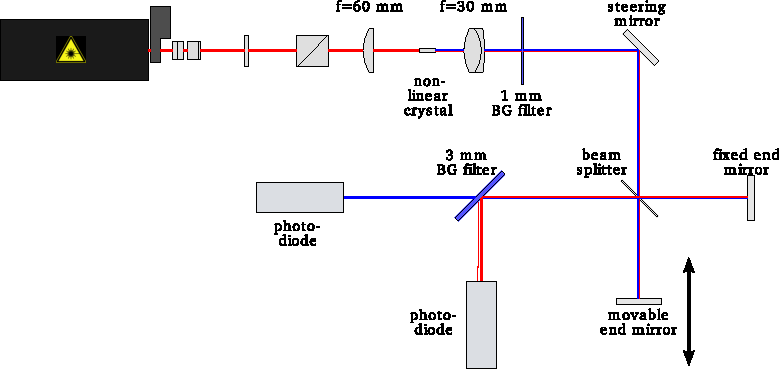
\includegraphics{fig-5}
    \caption{%
        %
    }
    \label{fig:fig-5}
\end{figure}

\end{document}

% vim: spell spelllang=en_us tw=79
